\subsection{Jet internal structure}\label{sec:jetsub}
The first measurements of jet quenching through full jet reconstruction at the LHC revolutionized our understanding of parton energy loss in a hot and dense medium. Nevertheless, there remains a gap in our understanding of the jet quenching mechanism that could be resolved by measuring the exact properties of the parton shower. High statistics of collected jets during HL-LHC will provide a prime opportunity to explore the details of the internal structure of high energy jets that undergo interactions with the QGP. Observables probing the internal structure of jets can be performed using all measured hadrons in a jet or by using subjet techniques selecting only a specific region of the radiation phase space. In the following sections both approaches and their potential will be discussed.

\subsubsection{Substructure with hadrons}
Inclusive measurements of the longitudinal and transverse momentum distribution of hadrons in inclusive jets have been performed with high acccuracy at the LHC \cite{Aaboud:2018hpb,Sirunyan:2018jqr}. The modification due to jet quenching is studied by comparing the results in pp and PbPb collisions. When interpreting these results one has to realize that by selecting on the jet momentum a different sample of partons initiating the jet is used in pp and PbPb collisions. This can be overcome by using jets recoiling from high momentum photons. The expected performance of the radial \pT\ profile in jets recoiling from a high momentum photon with at HL-LHC is shown in Fig.\ref{fig:jetshape}. The central values of the extrapolated spectra are obtained by smoothing the results from~\cite{Sirunyan:2018ncy} by a third order polynomial. The systematic uncertainties shown are obtained by reducing by a factor of two those from the 2015 PbPb data results, considering the expected improvements on the jet energy scale and jet energy resolution uncertainties. The results show that the photon-tagged jet shape could be measured with high precision and provide valuable insights about the modification of the jet transverse structure of quark initiated jets in the strongly interacting medium.
%
\begin{figure}[!ht]
\begin{center}
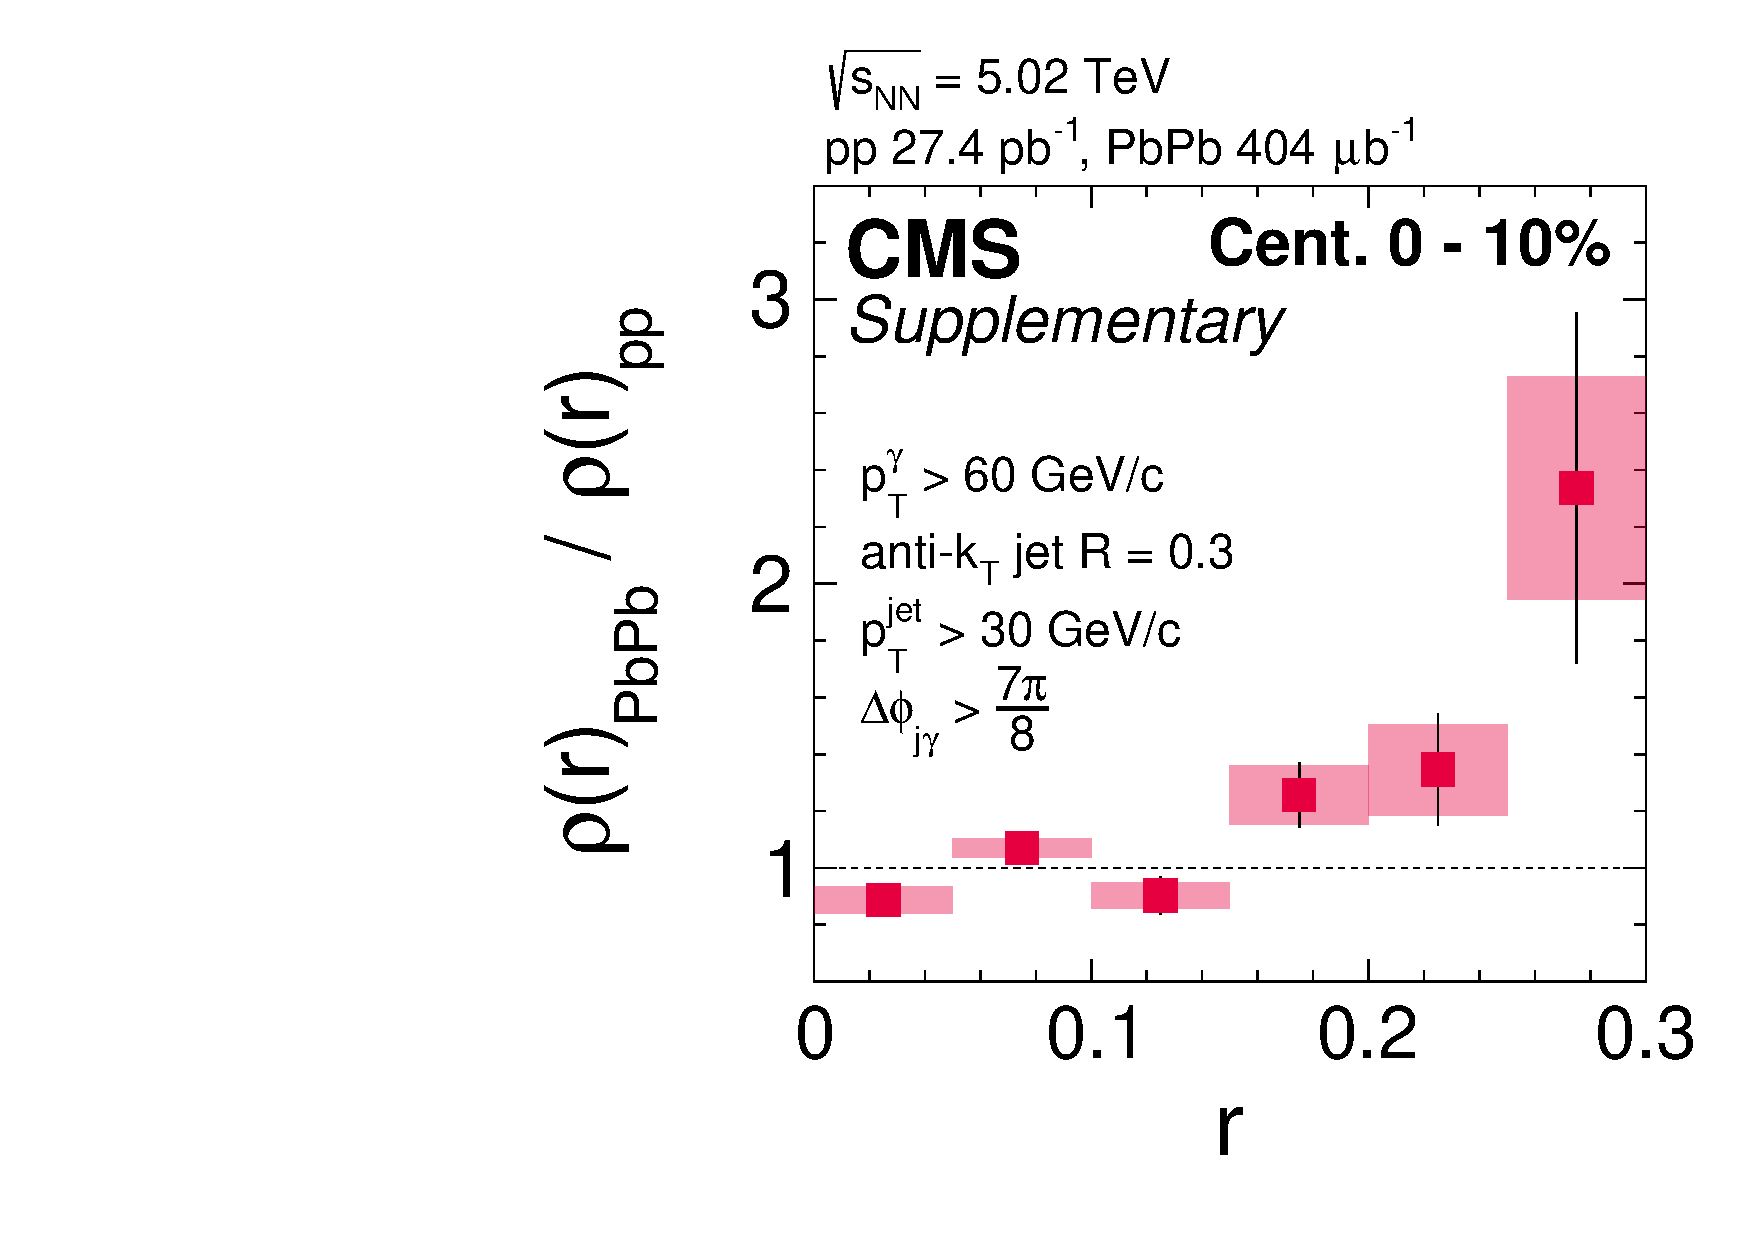
\includegraphics[width=.485\textwidth]{\main/jets/figures/cms/CMS-HIN-18-006_Figure-aux_004.pdf}
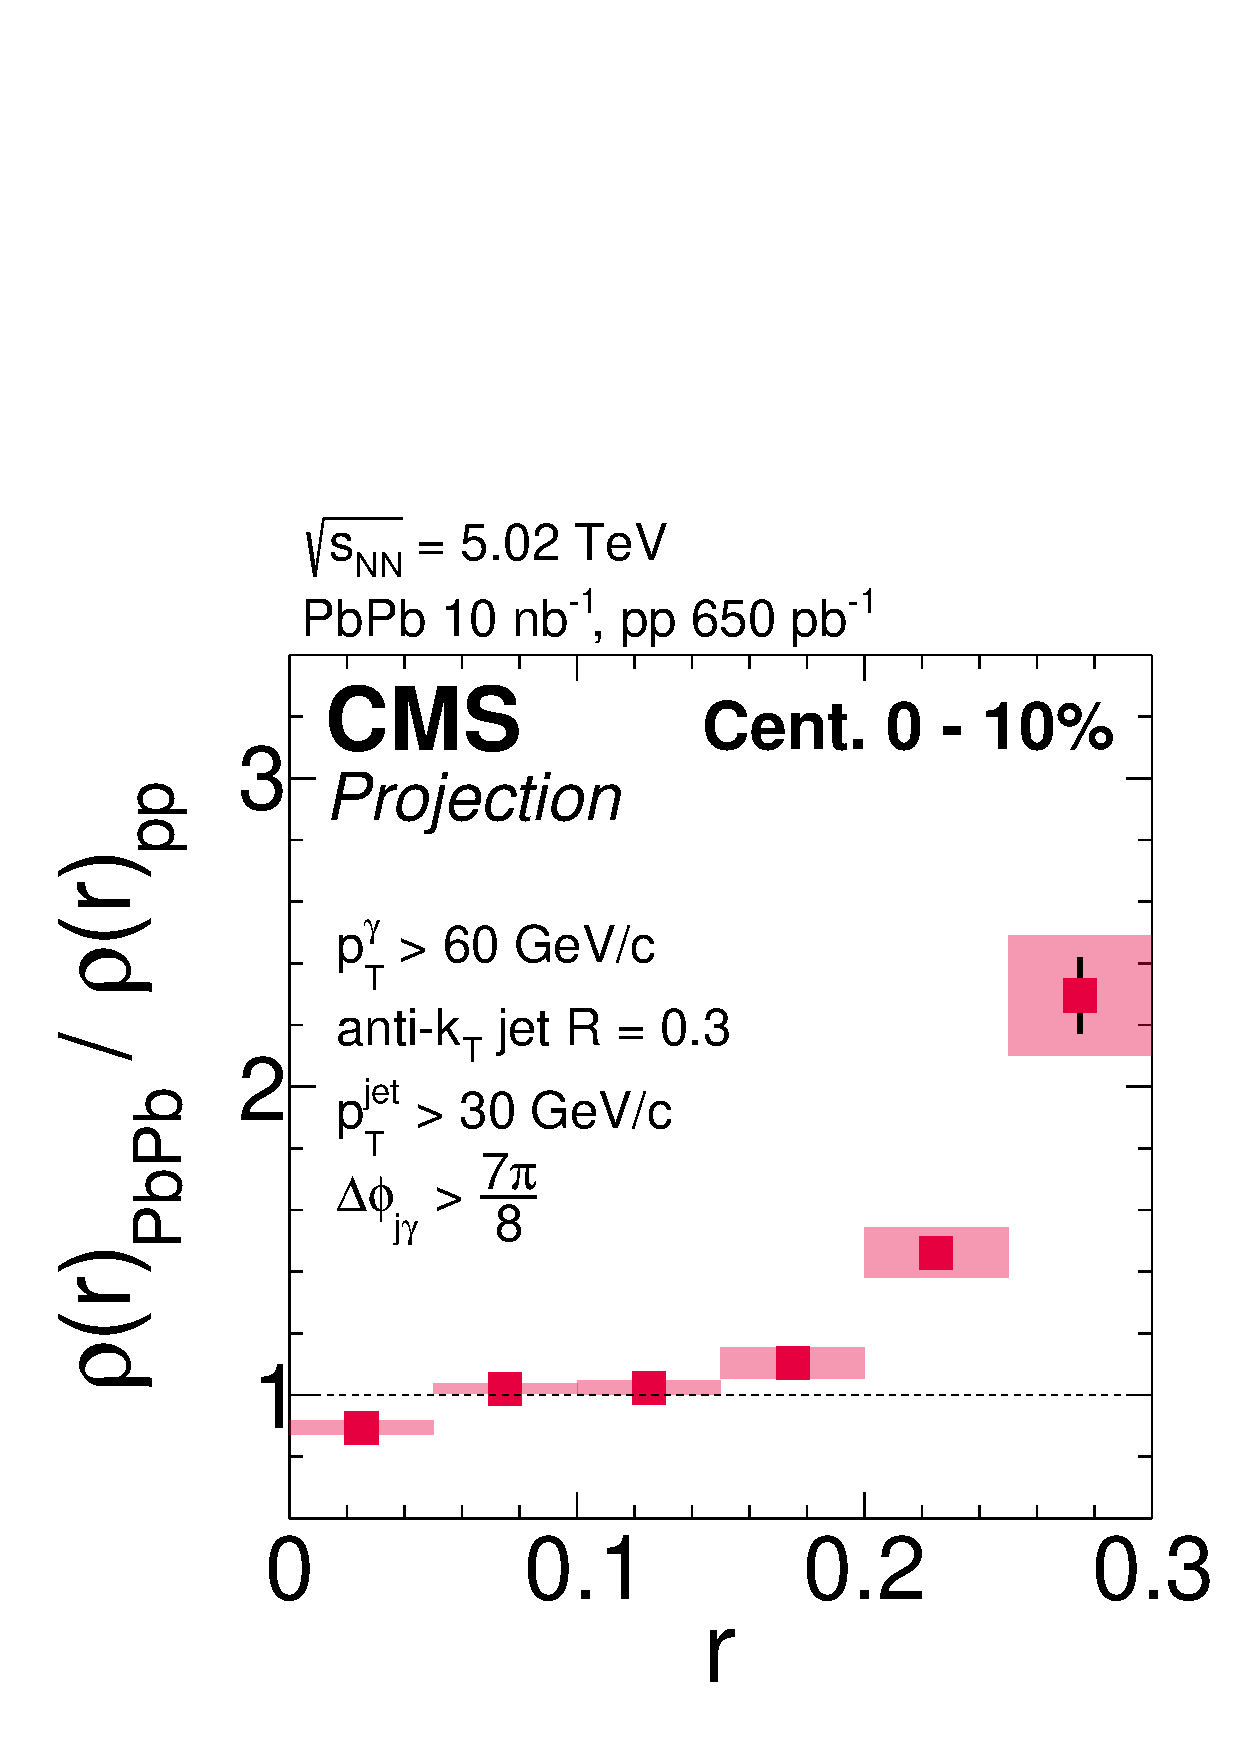
\includegraphics[width=.45\textwidth]{\main/jets/figures/cms/projection_js_ratioOnly_fit_pol3_sysReduced50Prct.pdf}
\caption{(Left Panel:) The ratio of measured photon-tagged jet shape in PbPb and pp collisions with the 2015 data. (Right Panel:) The expected performance of the jet shape ratio in the HL-LHC data, using a third-order polinomial for smoothing the data. [REF to be added when note is public]}
\label{fig:jetshape}
\end{center}
\end{figure}

[ATLAS projection for FF?]


\subsubsection{Substructure with subjets}
During the parton shower evolution, an early hard splitting will result in two partons with high transverse momentum separated in angle. Information about these leading partonic components can be obtained by removing the softer wide-angle radiation contributions. This is done through the use of jet grooming algorithms that attempt to split a single jet into two subjets, a process referred to as ``declustering''~\cite{Ellis:2009me,Butterworth:2008iy,Krohn:2009th,Dasgupta:2013ihk,Larkoski:2014wba}. For a parton shower in vacuum, these subjets provide access to the properties of the first splitting in the parton evolution~\cite{Altarelli:1977zs,Larkoski:2015lea}. Figure \ref{fig:ZG} shows the expected performance for the momentum sharing fraction, $z_{\mathrm{g}}$, in the HL-LHC phase. The central values of the extrapolated splitting function and jet mass are from previous CMS publications~\cite{Sirunyan:2017bsd,Sirunyan:2018gct}. The systematic uncertainties are reduced by a factor of two with respect to the results with 2015 PbPb data due to the expected improvements on the jet energy scale and jet energy resolution uncertainties. With the HL-LHC data, these jet substructure observables could be measured with unprecedented accuracy and provide important constraints on the magnitude of the correlated medium response and the parton energy loss mechanism. While the current data is not precise enough to constrain the medium properties further, the expected luminosity at the HL-LHC will allow to do this in more detail as can be observed from the different outcome of the BDMPS \cite{Mehtar-Tani:2016aco} and SCETg \cite{Chien:2016led} calculation when the medium density ($\hat{q}$ for BDMPS and $g$ for SCETg) is varied. In addition, the expected precision will also allow to determine the relevance of various physics phenomena as is shown for the role of coherence in Fig. \ref{fig:ZG} in the HT theoretical calculations \cite{Chang:2017gkt}. Figure \ref{fig:Mass} shows the expected performance for the groomed jet mass where the 2015 PbPb data already showed that jet quenching might cause an increase of high mass jets \cite{Sirunyan:2018gct} for which especially the increase in statistics at the HL-LHC will be benificial.
\begin{figure}[!ht]
\begin{center}
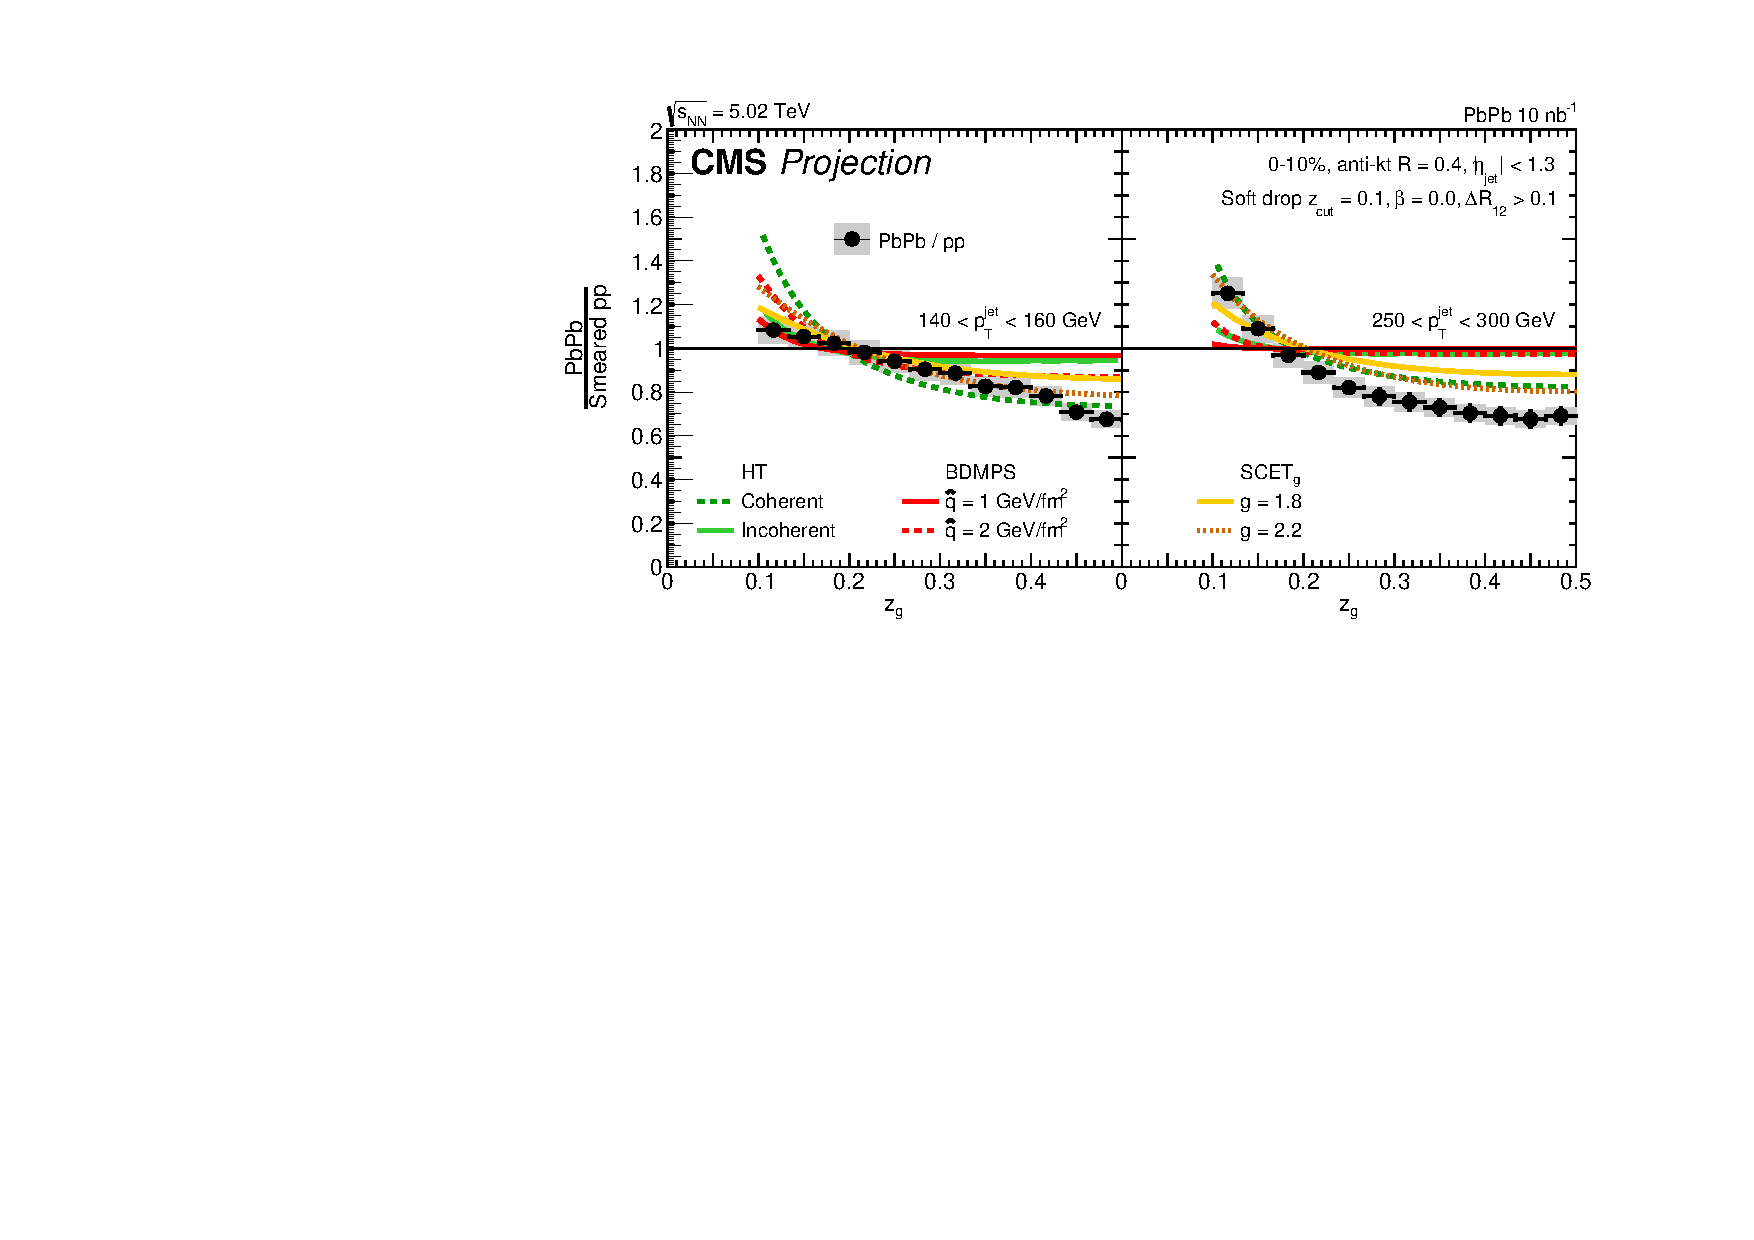
\includegraphics[width=.95\textwidth]{\main/jets/figures/cms/ZGMoneyPlot.pdf}
\caption{Performance of jet splitting function measurement with HL-LHC data in PbPb collisions for two different selections in jet transverse momentum. \cite{CMS-FTR-17-002:2017dec}}
\label{fig:ZG}
\end{center}
\end{figure}
%
\begin{figure}[!ht]
\begin{center}
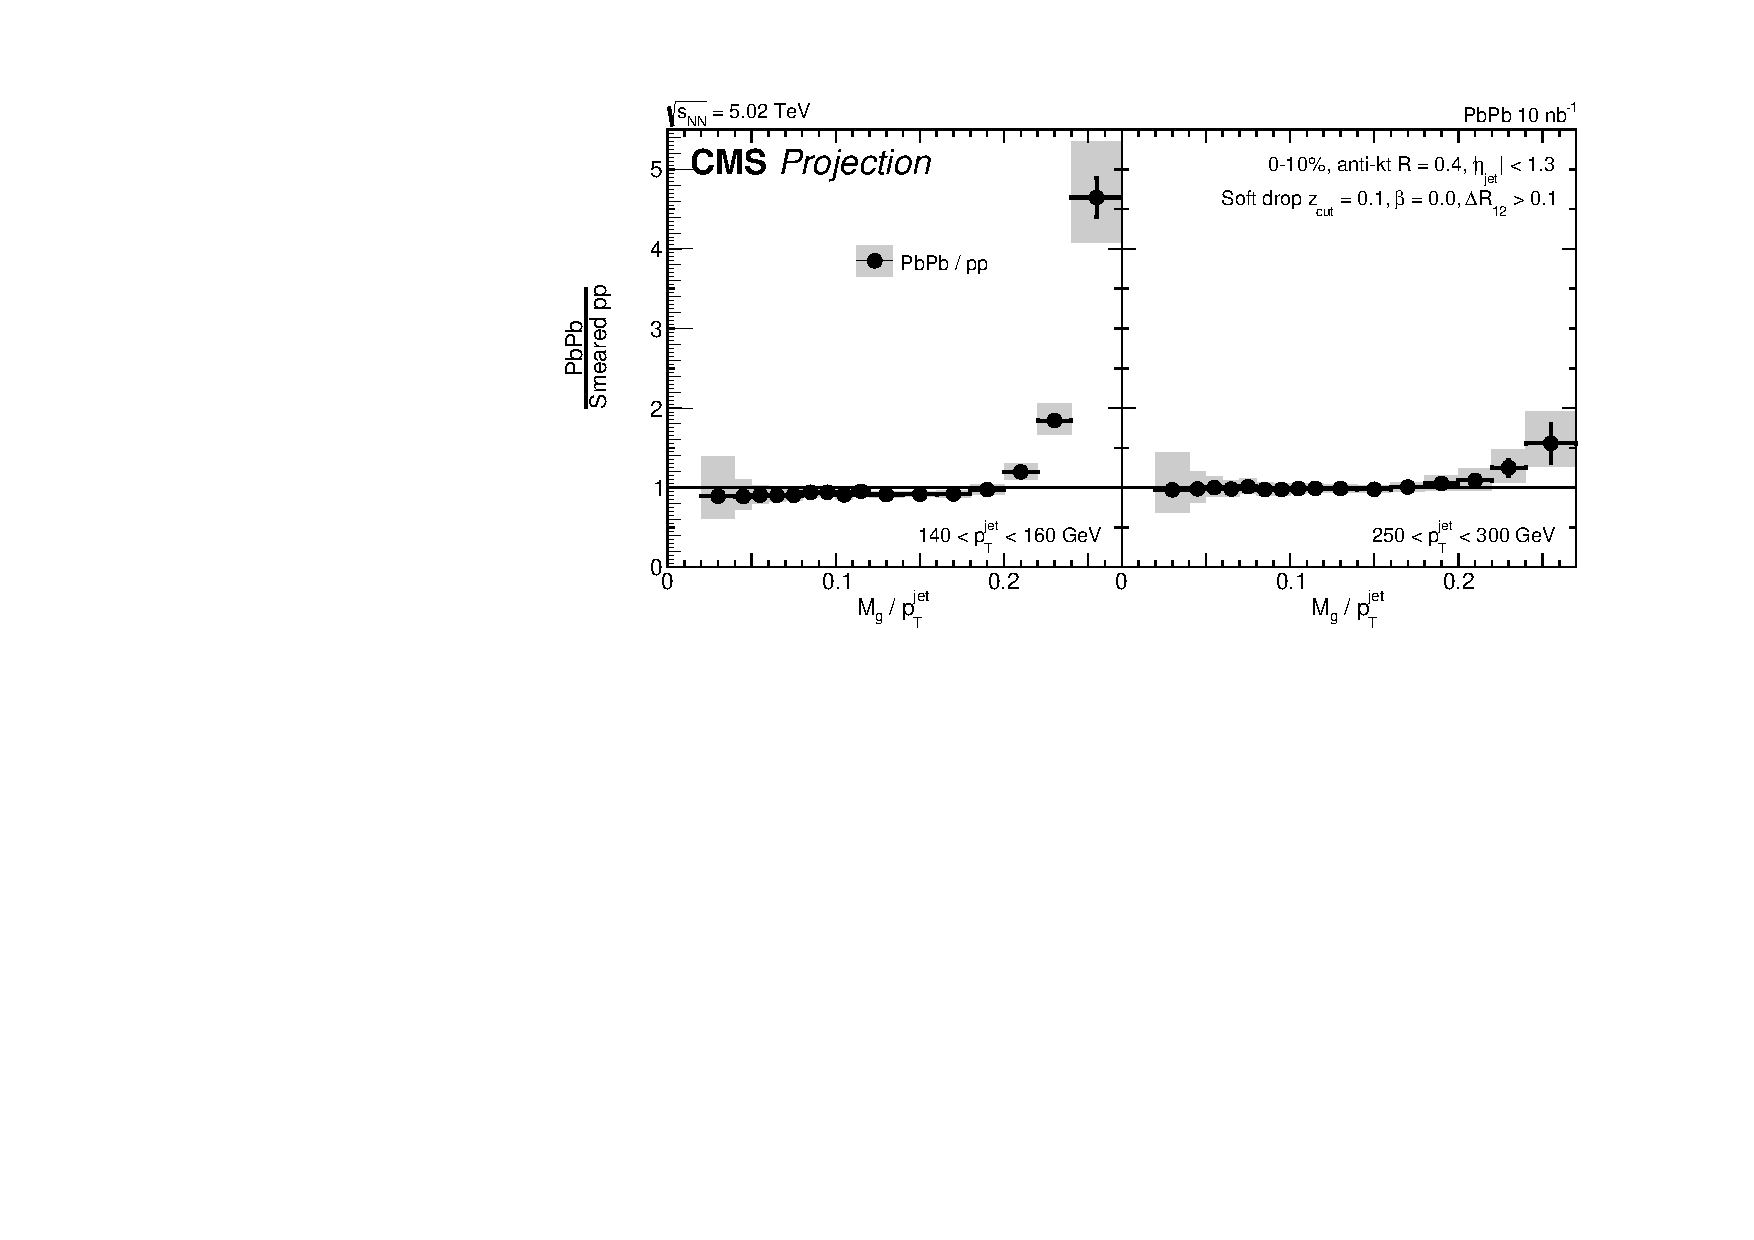
\includegraphics[width=.95\textwidth]{\main/jets/figures/cms/MGMoneyPlot_0.pdf}
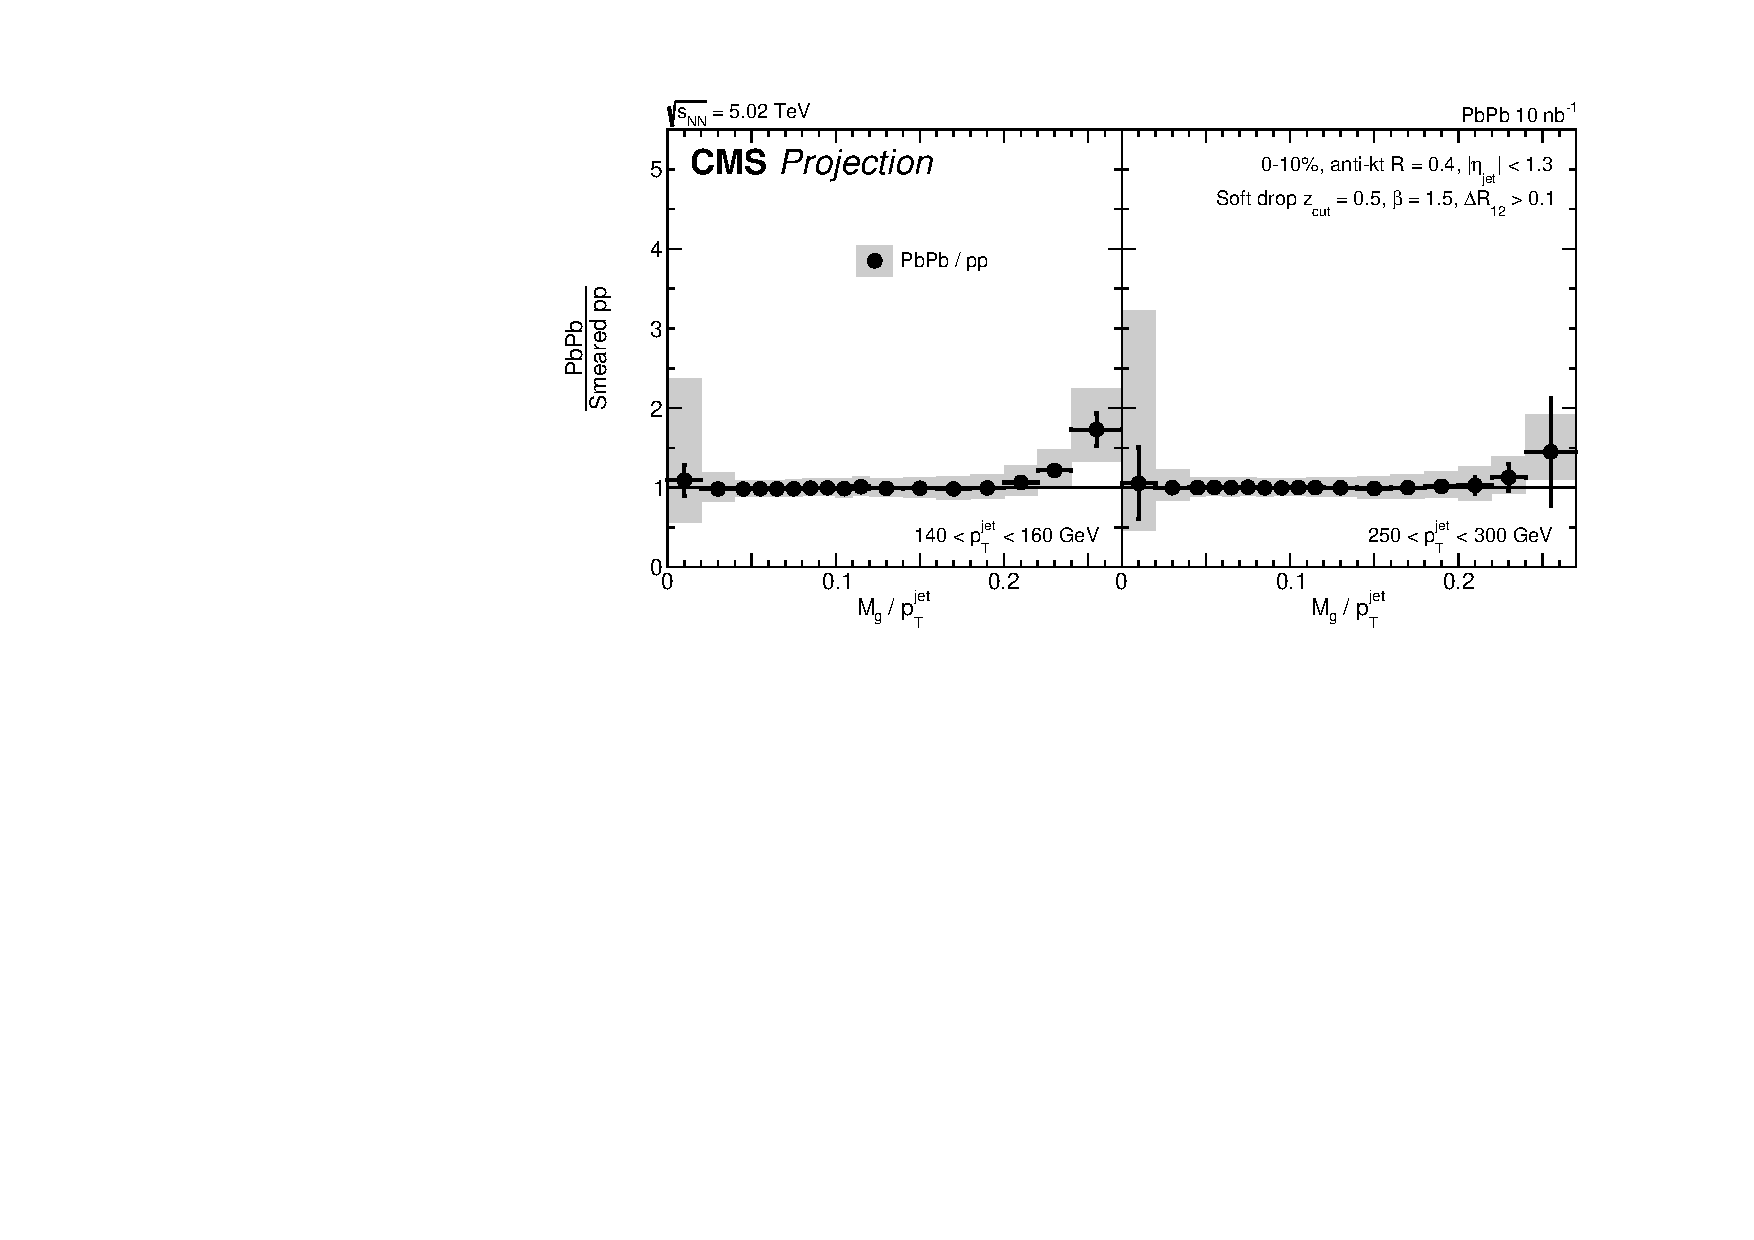
\includegraphics[width=.95\textwidth]{\main/jets/figures/cms/MGMoneyPlot_7.pdf}
\caption{Jet Mass distribution with grooming setting $(z_{cut},\beta)=(0.1,0.0)$ (Upper panels) and $(z_{cut},\beta)=(0.5,1.5)$ (Lower panels). \cite{CMS-FTR-17-002:2017dec}}
\label{fig:Mass}
\end{center}
\end{figure}


\newpage
\subsubsection{Radiation phase space with Lund diagram}

Recently, a theoretical representation of the radiation phase space within jets inspired by Lund diagrams \cite{Andersson:1988gp} has been proposed to study medium modification of the radiation pattern. The so-called Lund jet plane \cite{Dreyer:2018nbf} - a robust portrayal of the internal structure of jets - was designed to build a conceptual connection between manually constructed observables and approaches that use Machine Learning techniques to study QCD jets and/or discriminate between signal and background jets.
The diagram is constructed by mapping the available phase-space within a jet to a triangle in a two dimensional (logarithmic) plane that shows the transverse momentum and the angle of any given emission with respect to its emitter.
Such a triangular diagram, a representation of the radiation within any given jet, can be created through repeated Cambridge/Aachen declustering.

To demonstrate the potential of future measurements at the LHC we constructed Lund diagrams using the \jewel\ Monte Carlo event generator \cite{Zapp:2013vla}.
To study the modifications of the Lund diagram with respect to a vacuum reference (jets produced in \pp\ collisions) we used the default settings of the generator corresponding to 10\% most central \PbPb\ collisions at the center of mass energy \sqrtsnn{5}.
The temperature of the medium was set to $T=0.42~\gev$ and the optional calculation of the so-called medium response retaining the partons / scattering centers that interacted with the jet was not used (i.e. {\it recoils off} setting of the MC generator was used).
Jets were reconstructed with the \akt\ algorithm \cite{Cacciari:2008gp} with resolution parameter $R=0.4$ using \fastjet\ package \cite{Cacciari:2011ma,Cacciari:2005hq}.
Jets retained for the substructure analysis were required to have their centroid within two units of pseudorapidity around $\eta_{\rm lab}=0$ (i.e. $|\eta^{\rm jet}| < 2$).
The substructure of jets was analyzed by reclustering the constituents of the jet with the Cambridge/Aachen (C/A) algorithm as implemented in \fastjet\ for two selections of jet \pt\ $80-120~\gevc$ and $200-250~\gevc$.

\begin{figure}[htbp]
	\centering
	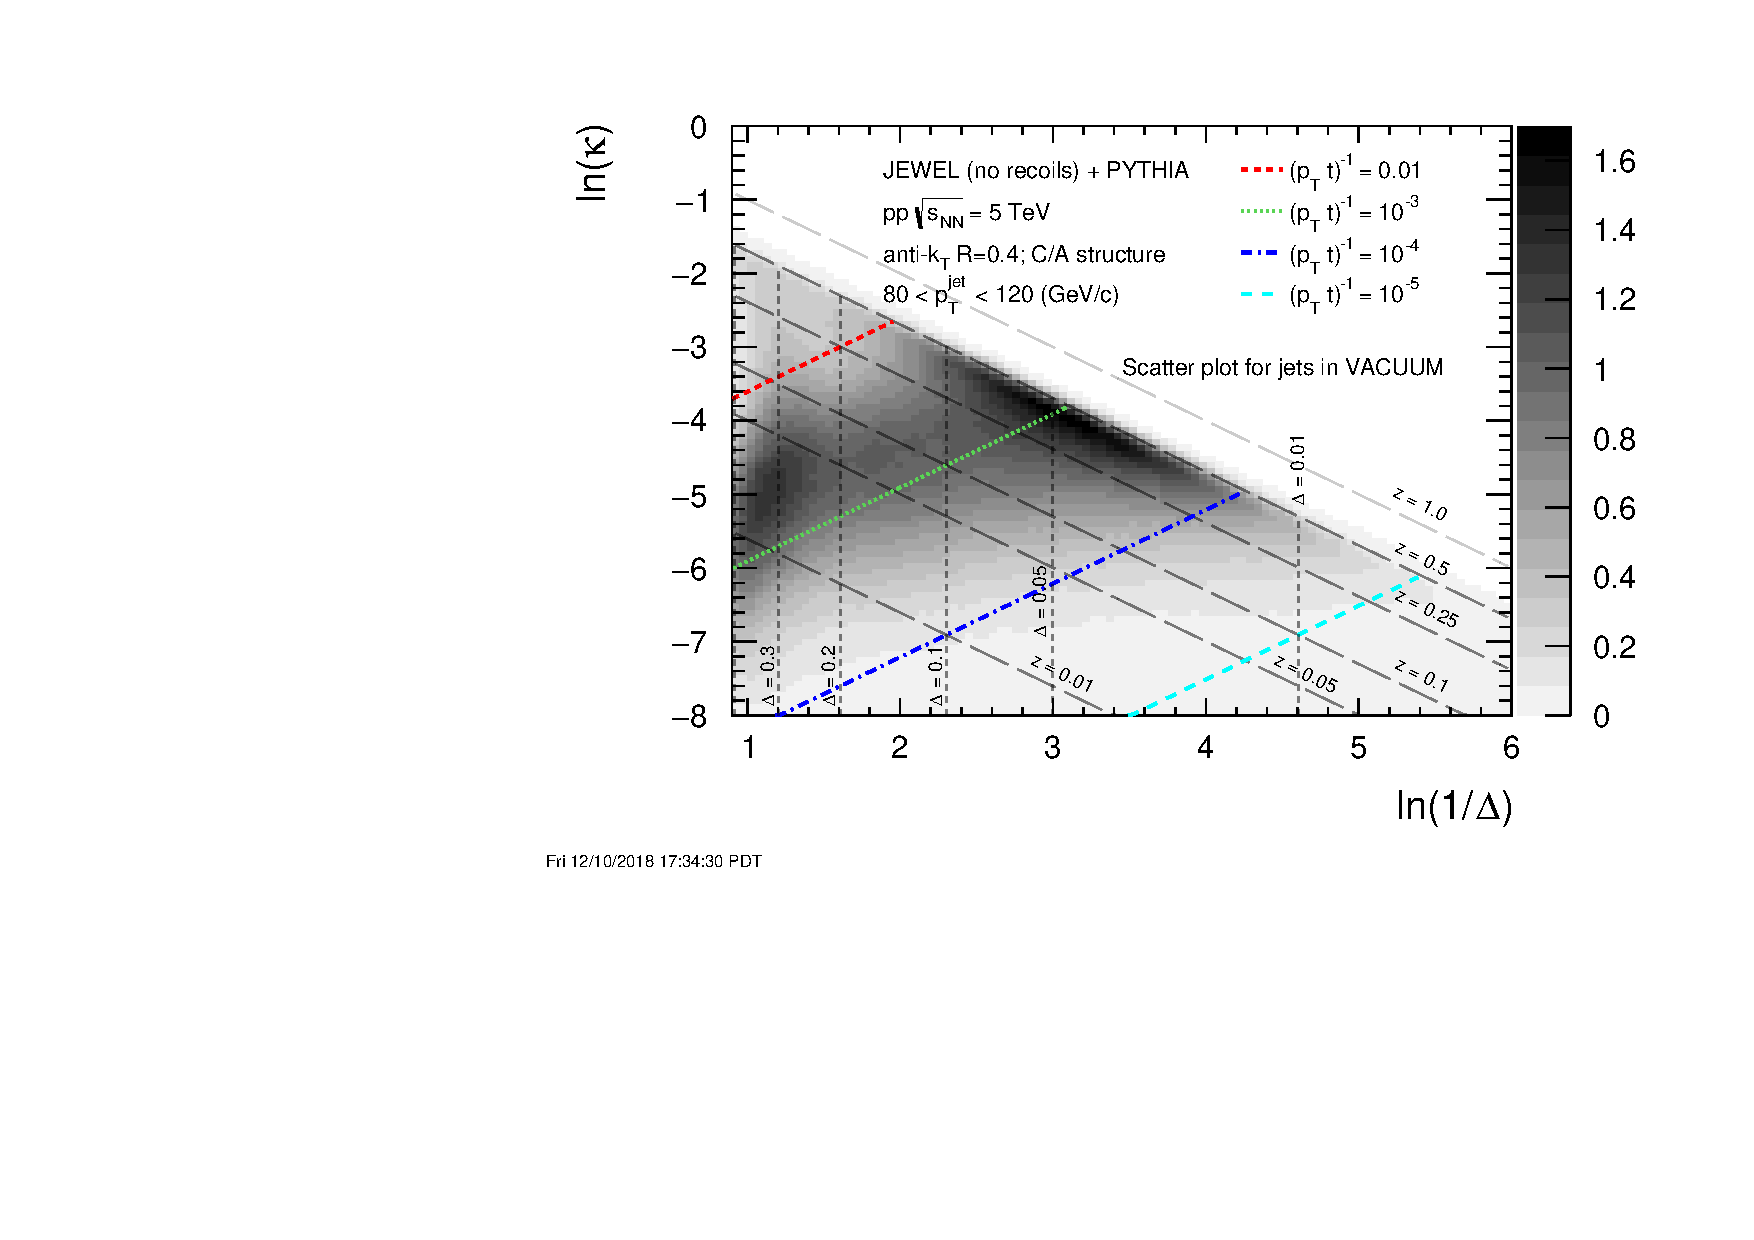
\includegraphics[width=0.45\textwidth,page=1]{\main/jets/figures/lund/lund_t}
	\includegraphics[width=0.45\textwidth,page=2]{\main/jets/figures/lund/lund_t}
	\includegraphics[width=0.45\textwidth,page=4]{\main/jets/figures/lund/lund_t}
	\includegraphics[width=0.45\textwidth,page=5]{\main/jets/figures/lund/lund_t}
	\caption{The density of points of a Lund diagram for anti-\kT\ $R=0.4$ jets for two \pt\ selections: $80 < \pt\ < 120$ \gevc\ in the upper row and $200 < \pt\ < 250$ \gevc\ in the lower row. Result of the JEWEL+PYTHIA Monte Carlo generator with left column: jets in \pp\ collisions; Right column: jets from \PbPb\ collisions - some with in-medium modifications. Each of the density plots shows curves of the average quantities of the densities over the other axis.}
	\label{fig:Lund_jets}
\end{figure}

The Lund diagram density can be directly measured experimentally and compared to analytic predictions and parton-shower Monte-Carlo simulations, such as \jewel.
Figure \ref{fig:Lund_jets} shows the density $\bar{\rho}$ of points (emissions) for a Lund diagram using the dimensionless quantity $\kappa$ and spatial separation of two emitters $\Delta$ within a jet (sub-)cluster following formulations in \cite{Dreyer:2018nbf}, such that
\begin{equation}
\bar{\rho}(\Delta, \kappa) = \frac{1}{N_{\rm jet}} \frac{dn_{\rm emission}}{d \ln \kappa~d \ln 1/\Delta},
\end{equation}
where for two clusters $a$ and $b$ labeled such that $p_{T,a} > p_{T,b}$, $\kappa=\frac{p_{T,b}}{p_{T,a} + p_{T,b}}\Delta_{ab}$, and $\Delta_{ab}^{2} = (y_a - y_b)^2 + (\varphi_a - \varphi_b)^2$ with $\varphi$ being the azimuthal angle and $y$ the rapidity of a cluster.
The $z_{g}$ variable which was defined in \cite{Larkoski:2015lea} and studied in heavy-ion collisions \cite{Sirunyan:2017bsd} is related to the variables in the Lund plane in the following way: $z_{\mathrm{g}} = \kappa/\delta$; lines of constant $z_\mathrm{g}$ are diagonals with negative slope in the Lund diagram. Note that since we re-cluster jets already reconstructed with \akt\ $R=0.4$ the angular separation between clusters within the jet is limited to $\ln 1/\Delta > 0.9$.

\begin{figure}[htbp]
	\centering
	\includegraphics[width=0.45\textwidth,page=3]{\main/jets/figures/lund/lund_t}
	\includegraphics[width=0.45\textwidth,page=6]{\main/jets/figures/lund/lund_t}
	\caption{Result of the JEWEL+PYTHIA MC simulation: MEDIUM-VACUUM difference of the calculations shown in Fig. \ref{fig:Lund_jets} for two jet \pt\ selections.}
	\label{fig:Lund_jets_vac_med}
\end{figure}

\textit{MvL: this text is to some extent repeated at the start of the 'Projection along angular separation' section; could refer to Fig 5 already here?}
The average density integrated over $\ln \kappa$ calculated for \PbPb\ (MEDIUM) case shows little deviation from the \pp\ (VACUUM) reference.
Whereas the average density along $\ln 1/\Delta$ for the MEDIUM case shows significant deviations from VACUUM for $\ln 1/\Delta < 3$ for jets in the lower \pt\ range and for $\ln 1/\Delta < 4$ for higher \pt\ jets.
These observations are consistent with soft and hard collinear splittings being modified by the medium.

\paragraph{Modifications of splittings and formation time}

{\it MP: text is a placeholder here...}
Following \cite{Andrews:2018jcm} we can divide the lund plane according to linear functions $\ln\kappa = \ln1/\Delta + \ln \frac{1}{p_{T} t}$, where $t$ is related to the decoherence time (thus formation time).
Depending on the selection, different formation times are probed and splittings will occur within or outside the medium.
We investigate three regions of the Lund plane according to a selection of diagonal lines for different $\frac{1}{p_{T} t}$ indicated in Fig. \ref{fig:Lund_jets}.
The density of the splittings is projected along the momentum imbalance $z = p_{T,b}/(p_{T,a} + p_{T,b})$.
In Fig. \ref{fig:Lund_projections_z} we show the relative difference of the splitting density $\Delta_{\rm}\bar{\rho} = (\bar{\rho}_{\mathrm med} - \bar{\rho}_{\mathrm vac})/\bar{\rho}_{\mathrm vac}$.
For small formation times the splitting density is suppressed for the in-medium calculations whereas for large $p_{T} t$ the modification is smaller and even slightly enhanced for large formation times.
This is consistent with the expectation that for large formation times the medium effects should be of smaller magnitude as compared to splittings formed early.

%\textit{MvL: Could we argue here that the reduction of splittings with short formation times is consistent with incoherent energy loss for partons that are produced inside the medium; i.e. pairs with short formation time lose more energy? }


\begin{figure}[htbp]
	\centering
	\includegraphics[width=0.3\textwidth,page=4]{\main/jets/figures/lund/lund_t_z}
	\includegraphics[width=0.3\textwidth,page=8]{\main/jets/figures/lund/lund_t_z}
	\includegraphics[width=0.3\textwidth,page=9]{\main/jets/figures/lund/lund_t_z}
	\caption{Projections of the relative difference of the Lund diagram onto momentum imbalance of the splittings for two selections of jet \pt\ and selections of $\frac{1}{p_{T} t}$.
	{\it Left:} relative difference for low-\pt\ jets for three selections of $\frac{1}{p_{T} t}$.
	{\it Middle:} relative difference for high-\pt\ jets for three selections of $\frac{1}{p_{T} t}$.
	{\it Right:} comparison of low- and high-\pt\ for two selections of $\frac{1}{p_{T} t}$.
	}
	\label{fig:Lund_projections_z}
\end{figure}

\paragraph{Projection along angular separation}
The most pronounced differences between VACUUM and MEDIUM calculations shown in Fig. \ref{fig:Lund_jets_vac_med} are visible for the region of $-3 < \ln \kappa < -3$ and large $\ln 1\Delta$ which correspond to the hard-collinear splittings (Region-A), and a band along $\ln 1/\Delta$ for small $\ln \kappa$ (Region-B): $-5 < \ln \kappa < -6$ for the lower \pt\ selection and $-5.5 < \ln \kappa < -7$ for higher \pt\ jets; that corresponds to an enhancement of soft (moderate $\ln 1/\Delta$) and hard collinear splittings (large $\ln 1/\Delta$).

\begin{figure}[htbp]
	\centering
	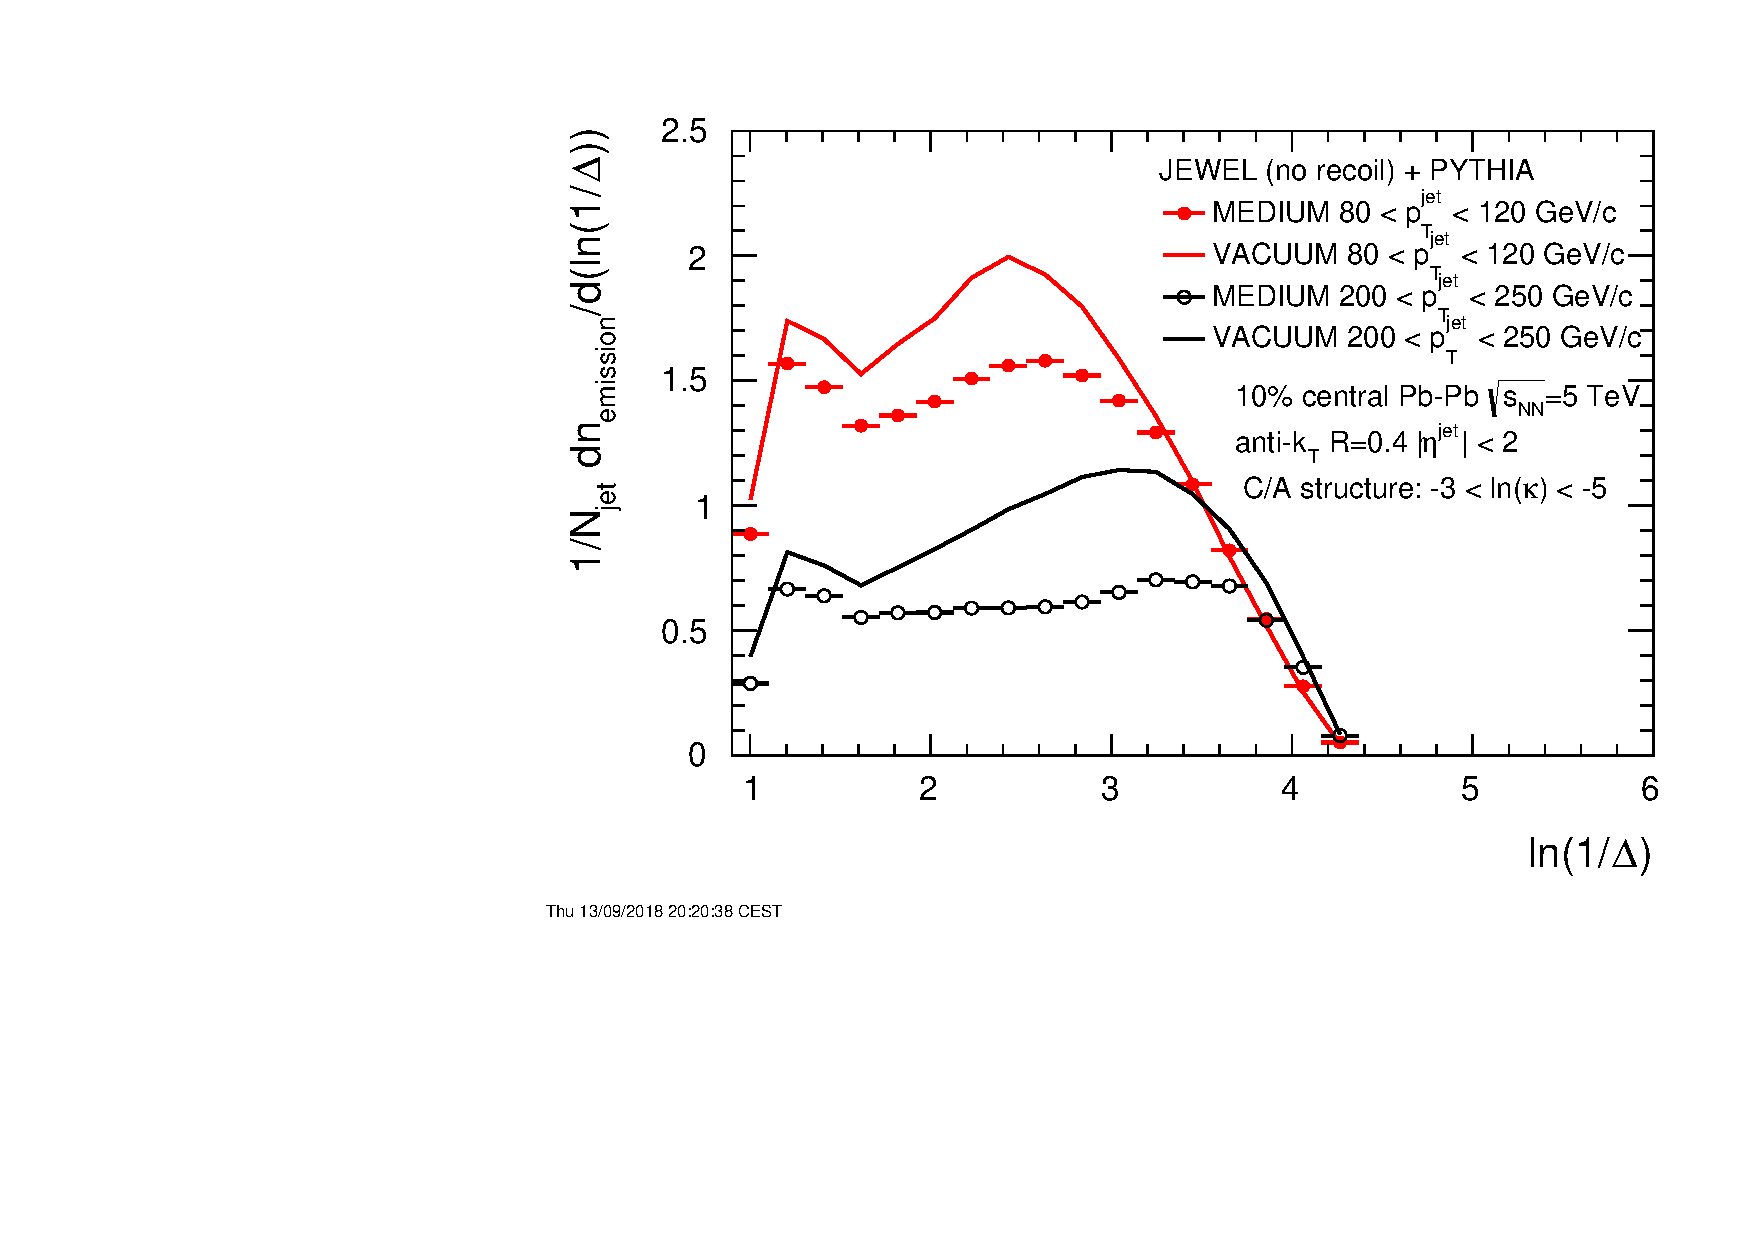
\includegraphics[width=0.45\textwidth,page=1]{\main/jets/figures/lund/lund_projections}
	\includegraphics[width=0.45\textwidth,page=2]{\main/jets/figures/lund/lund_projections}
	\caption{Projections of the lund diagram along the angular separation $ln 1/\Delta$ of the splittings for the two selections of jet \pt. In-medium suppression of splittings for moderate $\ln{\kappa}$ according to JEWEL - left. Enhancement for small $\ln{\kappa}$ - right.}
	\label{fig:Lund_projections}
\end{figure}

To illustrate the different modifications of the Lund diagram density for the two regions, Fig. \ref{fig:Lund_projections} shows projections (slices) along $\ln 1/\Delta$. For Region-A we observe 30\%-40\% depletion of splittings for the MEDIUM case whereas in Region-B a moderate increase of splittings induced by the medium is visible. The depletion in Region-A is consistent with a collimation of jet structure observed in heavy-ion collisions \cite{Acharya:2018uvf,Sirunyan:2018jqr} - a suppression of hard splittings. The increase seen in Region-B is consistent with a small in-medium enhancement of splittings with moderate dependency on the angle of the splitting but favoring the soft colinear medium-induced radiation (moderate $ln 1/\Delta$).

%\paragraph{Connection to present measurements}
%
%Considering another illustration - connect to the present measurements of $z_{g}$ with [a] Soft Drop condition... Lund-D inclusive for all splittings is quite different than for the ones selected by SD...

%\begin{figure}[htbp]
%	\centering
%	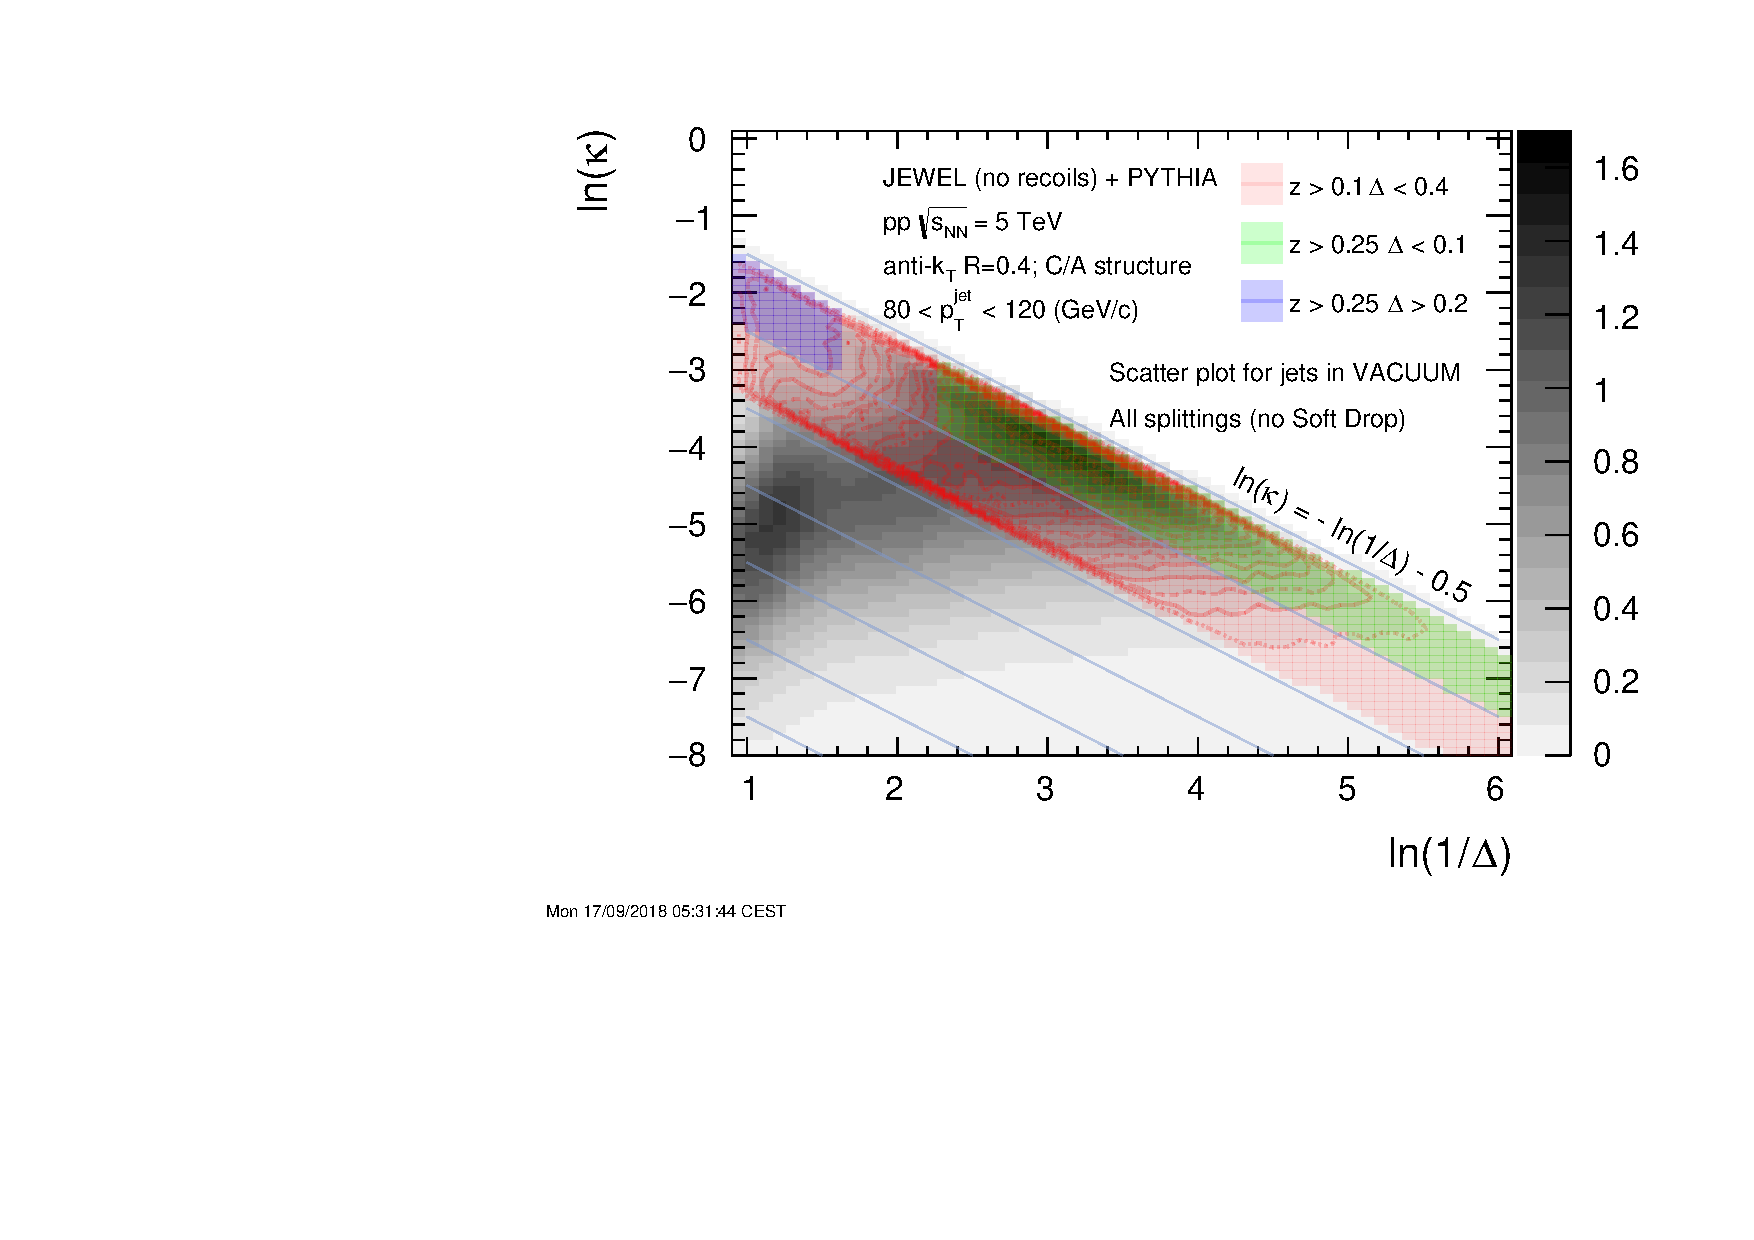
\includegraphics[width=0.45\textwidth,page=1]{\main/jets/figures/lund/lund_zg}
%	\includegraphics[width=0.45\textwidth,page=2]{\main/jets/figures/lund/lund_zg}
%	\includegraphics[width=0.45\textwidth,page=3]{\main/jets/figures/lund/lund_zg}
%	\includegraphics[width=0.45\textwidth,page=4]{\main/jets/figures/lund/lund_zg}
%	\caption{Lund diagram for 80-120 GeV/c jets with a few cut regions indicated; Lund for vacuum and medium for SD $z_{g}$ and the MEDIUM-VACUUM difference.}
%	\label{fig:Lund_zg_lowpt}
%\end{figure}
%
%\begin{figure}[htbp]
%	\centering
%	\includegraphics[width=0.45\textwidth,page=5]{\main/jets/figures/lund/lund_zg}
%	\includegraphics[width=0.45\textwidth,page=6]{\main/jets/figures/lund/lund_zg}
%	\includegraphics[width=0.45\textwidth,page=7]{\main/jets/figures/lund/lund_zg}
%	\includegraphics[width=0.45\textwidth,page=8]{\main/jets/figures/lund/lund_zg}
%	\caption{Lund diagram for 200-250 GeV/c jets with a few cut regions indicated; Lund for vacuum and medium for SD $z_{g}$ and the MEDIUM-VACUUM difference.}
%	\label{fig:Lund_zg_highpt}
%\end{figure}

%\subsection{Obsolete ?}

%\begin{figure}[htbp]
%	\centering
%	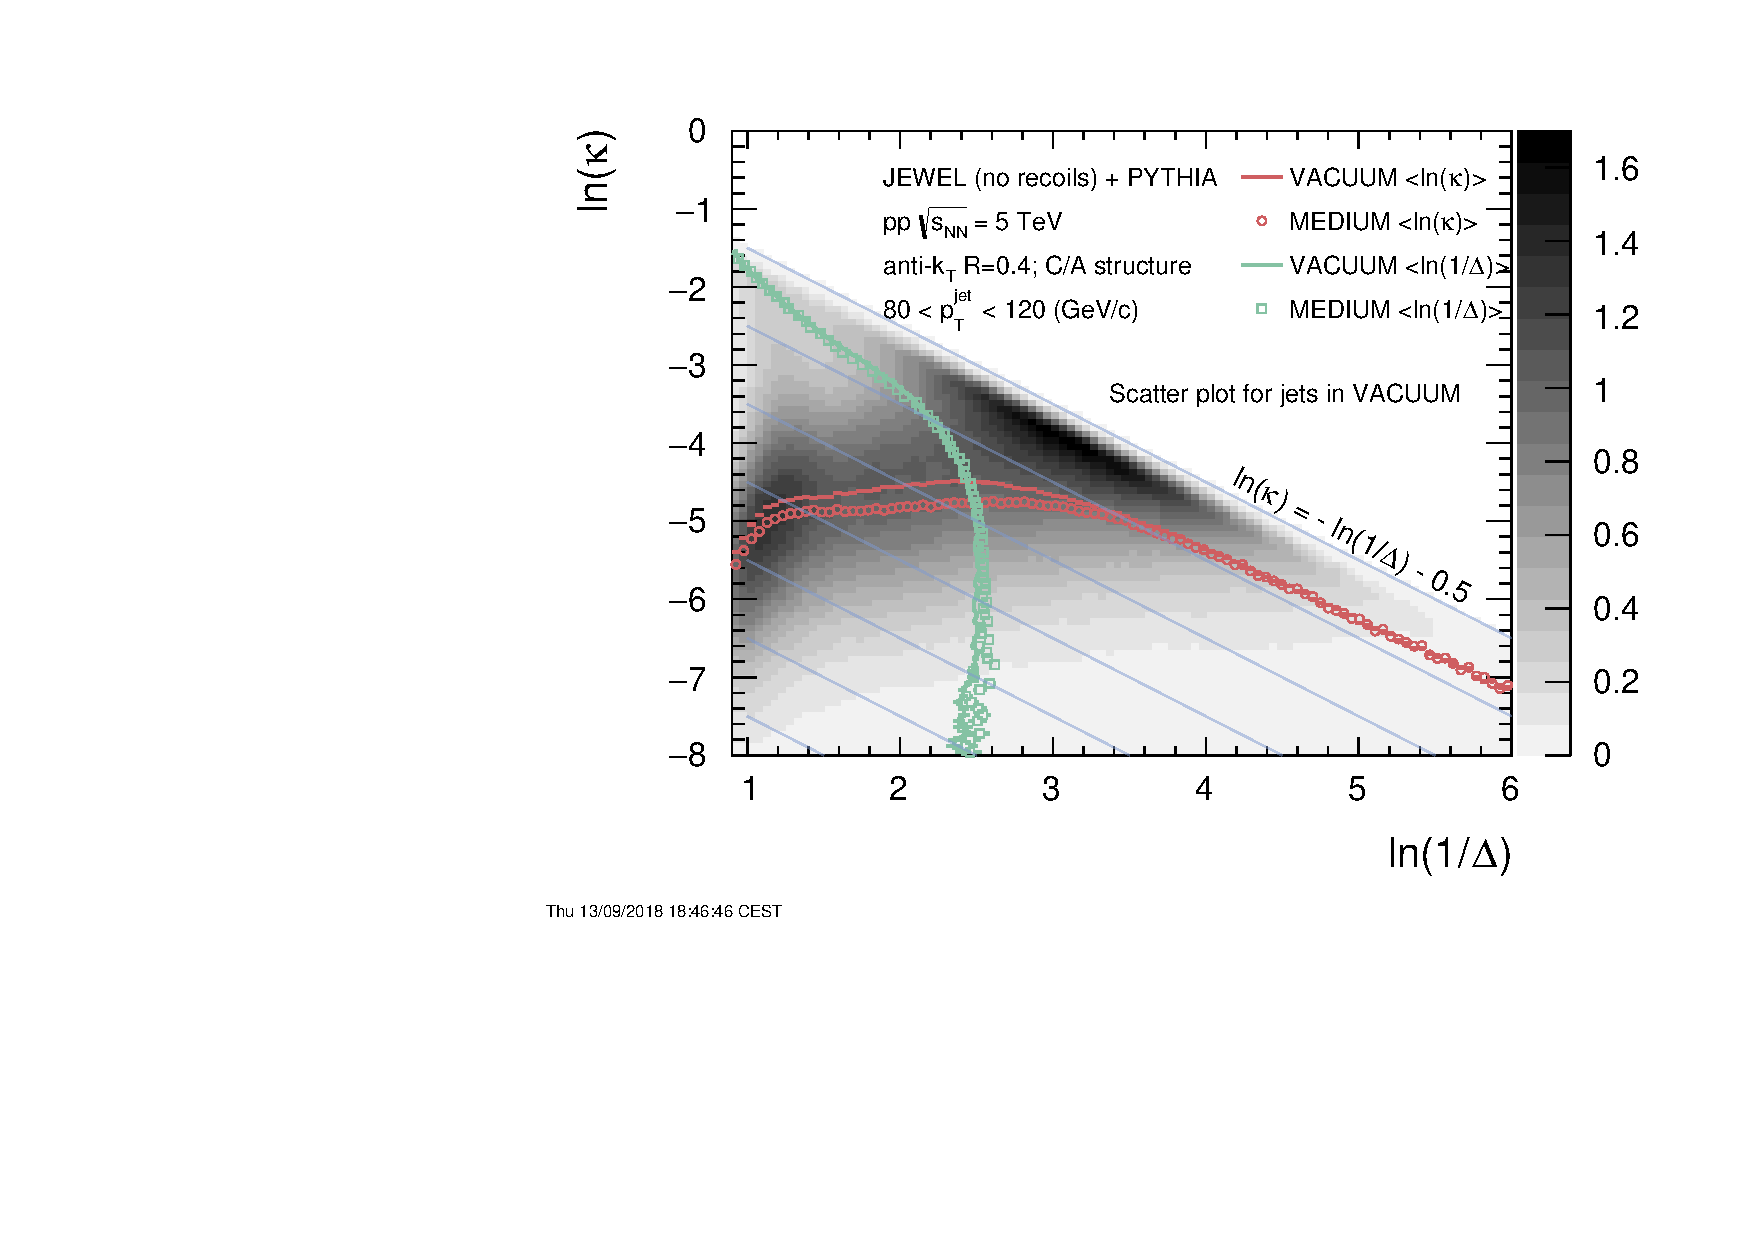
\includegraphics[width=0.45\textwidth,page=1]{\main/jets/figures/lund/lund}
%	\includegraphics[width=0.45\textwidth,page=2]{\main/jets/figures/lund/lund}
%	\includegraphics[width=0.45\textwidth,page=4]{\main/jets/figures/lund/lund}
%	\includegraphics[width=0.45\textwidth,page=5]{\main/jets/figures/lund/lund}
%	\caption{The density of points of a Lund diagram for anti-\kT\ $R=0.4$ jets for two \pt\ selections: $80 < \pt\ < 120$ \gevc\ in the upper row and $200 < \pt\ < 250$ \gevc\ in the lower row. Result of the JEWEL+PYTHIA Monte Carlo generator with left column: jets in \pp\ collisions; Right column: jets from \PbPb\ collisions - some with in-medium modifications. Each of the density plots shows curves of the average quantities of the densities over the other axis.}
%	\label{fig:Lund_jets}
%\end{figure}
